\documentclass[a4paper,12pt,titlepage]{article}
\usepackage[utf8]{inputenc}
\usepackage{graphicx} % Required for inserting images
\usepackage[spanish,es-tabla]{babel}
\usepackage[none]{hyphenat}
\usepackage[justification=centering]{caption}
\usepackage{subcaption}
\usepackage{amssymb, amsmath}
\usepackage{gensymb}
\usepackage{fancyhdr}
\usepackage{wrapfig}


\title{Giroscopio}
\author{Gonzalo Bastos González}

\usepackage[a4paper]{geometry}
\geometry{top=2cm, bottom=2.0cm,left=2cm, right=2cm}

\begin{document}

\begin{center}
    \textbf{\Large Giroscopio}
\end{center}

\begin{center}
    \textbf{Gonzalo Bastos González}
\end{center}

\section{Estudio del movimiento del giroscopio}

En primer lugar vamos a estudiar el movimiento del giroscopio y como responde a la aplicación de fuerzas externas. La ecuación del movimiento de un giroscopio es:

\begin{equation}
    \frac{d\vec{L}}{dt} = \vec{N} = \vec{r}\times\vec{F}
    \label{Ec movimiento}
\end{equation}

Para verificar esta relación vamos a aplicar un torque externo $\vec{N}$ y estudiaremos la respuesta del giroscopio. En concreto vamos a observar que dirección toma el vector variación del momento angular ($d\vec{L}$), que es paralelo al torque. Este vector indica en que sentido gira el giroscopio al aplicar la fuerza. En las siguientes figuras podemos ver un diagrama de fuerzas de las situaciones estudiadas.

\begin{figure}[h!]
    \centering
    \begin{subfigure}{0.45\textwidth}
        \centering
        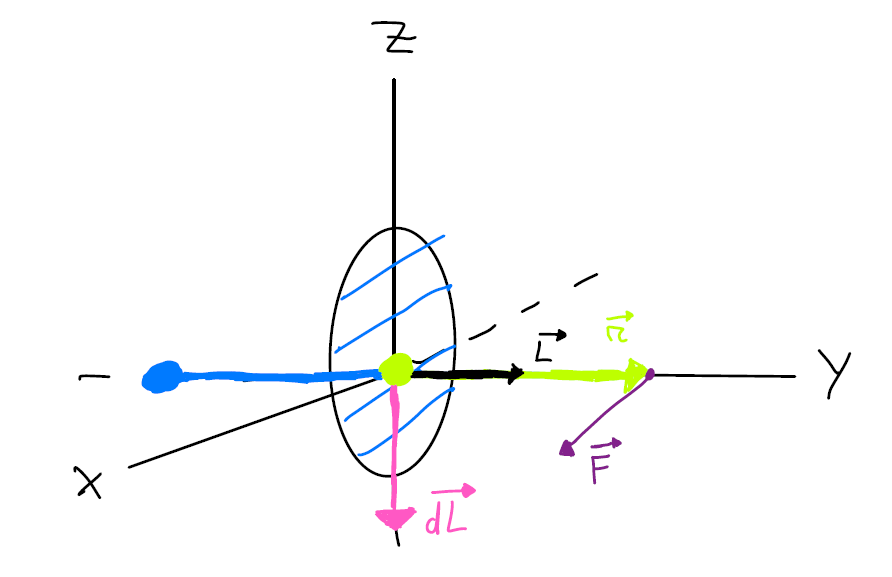
\includegraphics[width=0.95\linewidth]{Images/F(+x).png}
        \subcaption{$\vec{F}=F\hat{x}$}
    \end{subfigure}
    \begin{subfigure}{0.45\textwidth}
        \centering
        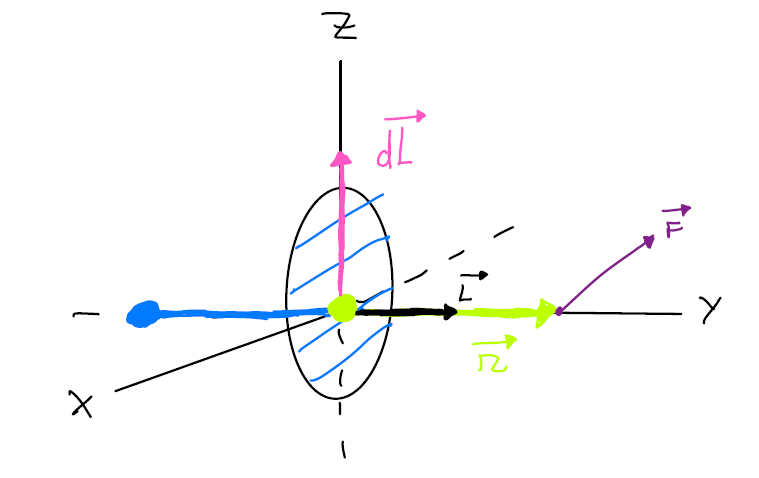
\includegraphics[width=.95\linewidth]{Images/F(-x).png}
        \subcaption{$\vec{F}=-F\hat{x}$}
    \end{subfigure}
    \caption{Respuesta del giroscopio a una fuerza en el eje $X$}
\end{figure}

\begin{figure}[h!]
    \centering
    \begin{subfigure}{0.45\textwidth}
        \centering
        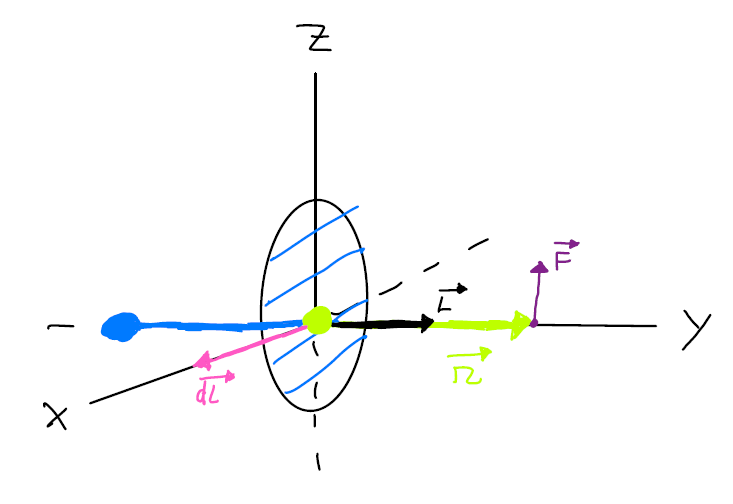
\includegraphics[width=0.95\linewidth]{Images/F(+z).png}
        \subcaption{$\vec{F}=F\hat{z}$}
    \end{subfigure}
    \begin{subfigure}{0.45\textwidth}
        \centering
        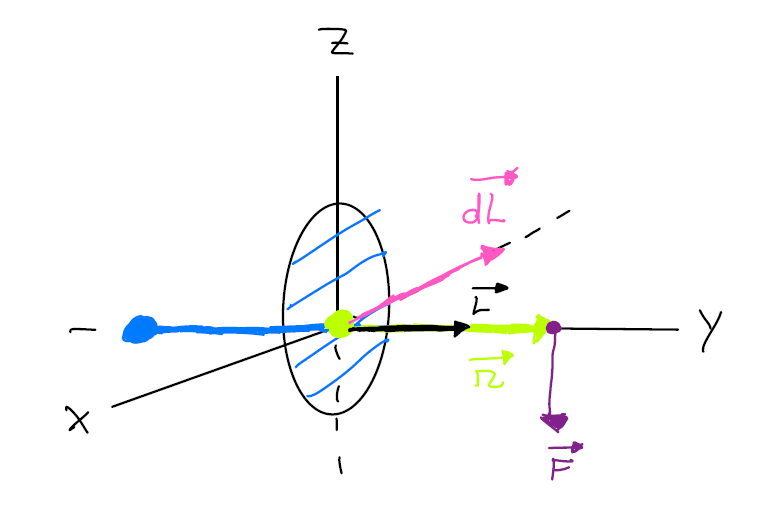
\includegraphics[width=.95\linewidth]{Images/F(-z).png}
        \subcaption{$\vec{F}=-F\hat{z}$}
    \end{subfigure}
    \caption{Respuesta del giroscopio a una fuerza en el eje $Z$}
\end{figure}

\newpage

\section{Momento de inercia respecto al eje de simetría}

Otro de los objetivos de la práctica es determinar el momento de inercia $I_3$ respecto al eje de rotación del giroscopio, que calcularemos mediante tres métodos:

\subsection{Valor teórico de $I_3$}

Definimos el momento de inercia de nuestro sólido rígido como:

\begin{equation}
    I = \int r^2 \,dm \Rightarrow I_3 = \int_{0}^{2\pi}\int_{0}^{R} \rho_s r^3\,drd\varphi = \frac{1}{2}MR^2 = 0,01415\pm 0,00011 \;kg\cdot m^2
\end{equation}

Donde $r = 12,75\pm 0,05 \;cm$ es el radio del disco, obtenido a partir del diámetro.

\subsection{Obtención directa de $I_3$ con el estudio de una caída libre}

Partimos de la Ec.\ref{Ec movimiento}, que aplicamos al torque que crea una masa en caída libre ($N=mrg$), donde $r$ es el radio del disco al que enrollamos el hilo que sujeta la masa en caída. 

\begin{equation}
    \dot{L}_3 = I_3\cdot \dot{\omega}_3 = I_3\frac{a}{r}=mrg
\end{equation}

La masa $m$ sigue un MRUA partiendo desde el reposo, por lo que su aceleración es:

\begin{equation}
    a = \frac{2h}{t^2}
\end{equation}

Donde $t$ es el tiempo para una caída desde una distancia $h$. Las incertidumbres son \newline$s(h)=0,1\;cm$ y $s(t)=0,25\;s$. Con esta relación podemos obtener la siguiente relación, que nos permitirá calcular $I_3$ a partir de un ajuste por mínimos cuadrados de $h$ frente a $t^2$:

\begin{equation}
    h = \frac{mgr^2}{2I_3}t^2
\end{equation}

\begin{figure}[h!]
    \centering
    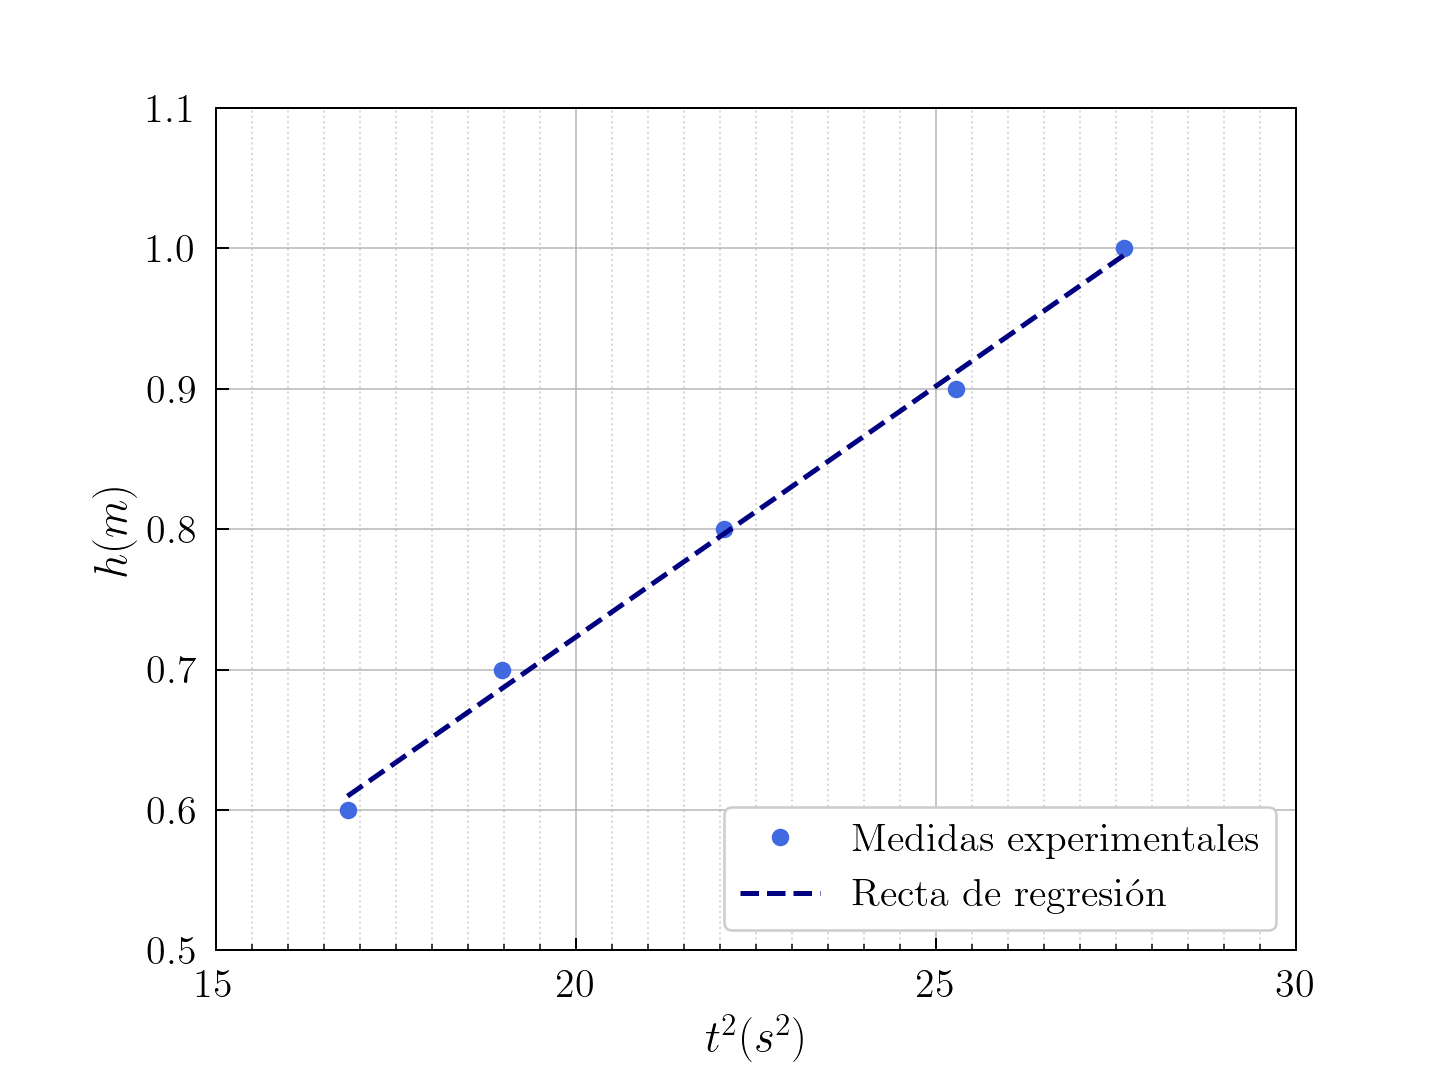
\includegraphics[width=0.65\linewidth]{Images/reg_h-t.png}
    \caption{Regresión lineal de $h$ frente a $t^2$}
\end{figure}

\newpage

Los resultados obtenidos de la regresión $h=a+bt^2$ son:

\begin{equation}
    \begin{gathered}
        a = 0,009 \pm 0,031 \;m\\
        b = 0,0357 \pm 0,0014 \;m\cdot s^{-2}\\
        r = 0,997
    \end{gathered}
\end{equation}

Como era de esperar el término independiente es despreciable, por lo que podemos calcular el valor de $I_3$ a partir de la pendiente de la recta de regresión:

\begin{equation}
    I_3 = \frac{mgr^2}{2b} = 0,00963 \pm 0,00053 \;kg\cdot m^2
\end{equation}

\subsection{Obtención de $I_3$ a partir del estudio del movimiento de precesión}

El movimiento de precesión es aquel que se produce cuando desequilibramos el giroscopio colgando una masa $m$ de su eje de giro, que creará un torque que modificará el momento angular, como sucedía en la primera parte de la práctica. El giroscopio girará con un periodo $T_p$ que está relacionado con su velocidad angular $\omega$ a partir de la siguiente ecuación:

\begin{equation}
    T_p = \frac{2\pi I_3}{mgd}\omega
    \label{Precesion}
\end{equation}

Donde $d$ es la distancia desde el centro de masas del giroscopio al punto de aplicación de la fuerza. Para comprobar esta relación realizamos tres series de cinco medidas cada una que nos permitirán realizar tres ajustes lineales a la Ec.\ref{Precesion}, obteniendo un valor medio de $I_3$ a partir de esos ajustes. Las incertidumbres son $s(T_p)=0,025\;s$, $s(\omega)=0,157 \;rad\cdot s^{-1}$, $s(m)=0,001\;kg$ y $s(d)=0,1\;cm$.

\begin{figure}[h!]
    \centering
    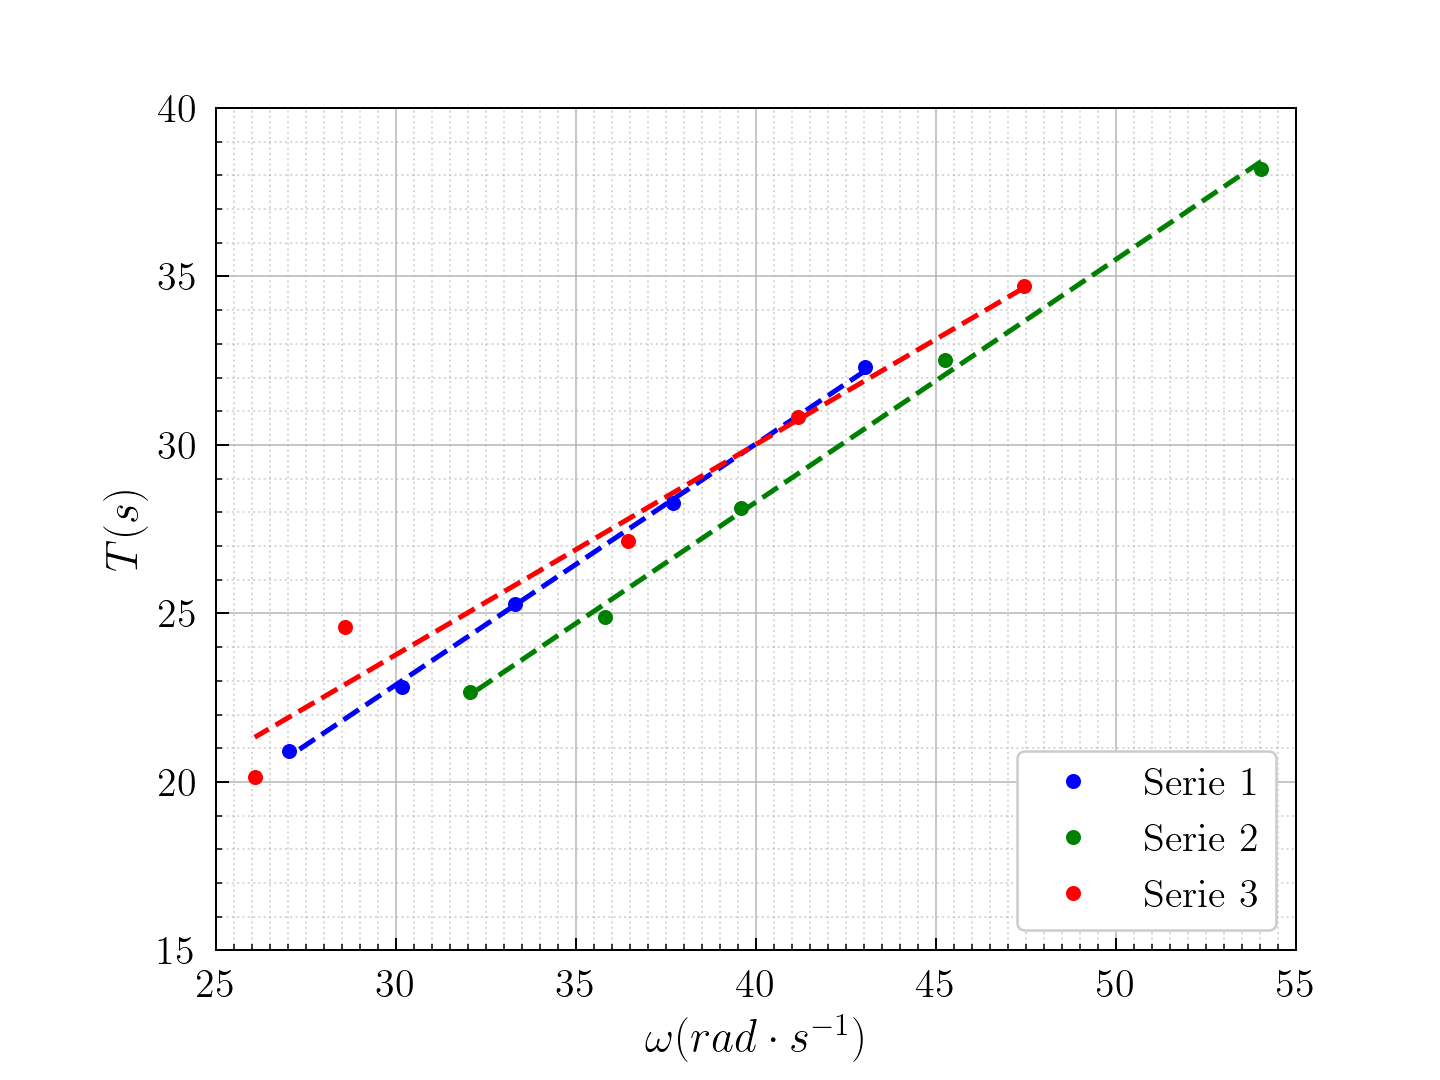
\includegraphics[width=0.75\linewidth]{Images/reg_precesion2.png}
    \caption{Regresión lineal de $T_p$ frente a $\omega$}
\end{figure}

\newpage

A partir de los parámetros de las regresiones podemos calcular los tres valores diferentes de $I_3$, a partir de los que calcularemos un valor medio:

\begin{table}[h!]
    \centering
    \begin{tabular}{|c|c|c|c|c|}
        \hline
        Parámetros & $a(s)$ & $b(s^2)$ & $r$ & $I_3(kg\cdot m^2)$ \\ \hline
        Serie 1 & $1,44 \pm 0,44$ & $0,715\pm 0,013$ & 0,9995 & $0,00483 \pm 0,00013$\\ \hline
        Serie 2 & $-0,50 \pm 0,93$ & $0,720 \pm 0,022$ & 0,998 & $0,00451 \pm 0,00017$\\ \hline
        Serie 3 & $5,0 \pm 2,6$ & $0,624 \pm 0,071$ & 0,98 & $0,00391 \pm 0,00045$\\ \hline
    \end{tabular}
    \caption{Parámetros obtenidos a partir de los ajustes}
\end{table}

Calculando la media ponderada de estos valores tenemos que:

\begin{equation}
    I_3 = 0,00447 \pm 0,00010 \;kg\cdot m^2
\end{equation}

\section{Momento de inercia respecto a un eje perpendicular al de simetría}

Una vez determinado el momento $I_3$ respecto al eje de simetría otro de los objetivos de la práctica era determinar el momento de inercia respecto a un eje perpendicular al de simetría, $I_1$, que calcularemos mediante tres métodos también.

\subsection{Valor teórico}

Para calcular el valor teórico de $I_1$ vamos a suponer que todas las masas que actúan son puntuales, obteniendo la siguiente ecuación:

\begin{equation}
    I_1 = \sum r_i^2m_i = MD^2+md^2
\end{equation}

Donde $M$ es la masa del disco, $m$ es la masa del contrapeso y $D$ y $d$ son las respectivas distancias al eje en donde queremos calcular el momento de inercia. Obtenemos por tanto un valor teórico de:

\begin{equation}
    I_1 = 0.0625 \pm 0,0059 \;kg\cdot m^2
\end{equation}

\subsection{Oscilaciones con resortes}

En esta parte conectaremos nuestro giroscopio a dos muelles verticales colgados de un soporte y pondremos a oscilar el sistema, que seguirá un movimiento armónico de frecuencia:

\begin{equation}
    \omega_1 = \sqrt{\frac{2k}{I_1}}D
    \label{k}
\end{equation}

Donde $D$ es la longitud del brazo de par, desde el eje de aplicación hasta el punto de aplicación de los resortes, y $k$ es la constante de los muelles, que suponemos iguales. En primer lugar tenemos que determinar la constante $k$ por el método dinámico a partir de la siguiente ecuación:

\begin{equation}
    k = \frac{4\pi^2m}{T^2} = 20,28 \pm 0,49 \;N\cdot m^{-1}
\end{equation}

Las incertidumbres son $s(m)=0,001\;kg$ y $s(T)=0,05\;s$. Una vez obtenido el valor de $k$ podemos calcular $I_1$ empleando la Ec.\ref{k}:

\begin{equation}
    I_1 = \frac{2kD^2}{\omega_1^2}
\end{equation}

Para calcular $\omega_1$ medimos el tiempo de 10 oscilaciones, calculamos el periodo y con eso podemos saber la frecuencia de oscilaciones $\omega_1$. Con este valor ya podemos calcular $I_1$:

\begin{equation}
    I_1 = 0,0791 \pm 0,0093 \;kg\cdot m^2
\end{equation}

Donde la incertidumbre de la distancia $D$ es $s(D)=0,1\;cm$.

\subsection{Estudio del movimiento de nutación}

Cuando desequilibramos nuestro giroscopio en rotación dándole un pequeño golpe en el extremo del eje se produce un movimiento periódico de cabeceo denominado nutación. Este movimiento obedece a la siguiente ecuación:

\begin{equation}
    \Omega_n = \frac{I_3}{I_1}\omega
\end{equation}

Donde $\Omega_n$ es la frecuencia de nutación ($s(\Omega_n)=\frac{2\pi}{t^2}$) y $\omega$ la frecuencia de giro con \newline$s(\omega)=1,57\;rad\cdot s^{-1}$. Para el ajuste despreciamos la incertidumbre de $\omega$ y suponemos que $s(\Omega_n$) es constante, aunque representaremos su valor en cada punto en la gráfica. Midiendo pares de valores $\Omega_n$ y $\omega$ podemos realizar una regresión lineal y calcular $I_1$ a partir de la pendiente de la recta de regresión. Para medir $\Omega_n$ vamos a calcular el tiempo de cuatro cabeceos y obtendremos $T_n$, a partir de eso es sencillo obtener la frecuencia ($T_n=\frac{2\pi}{\Omega_n}$). Los valores obtenidos a partir del ajuste fueron los siguientes:

\begin{figure}[h!]
    \centering
    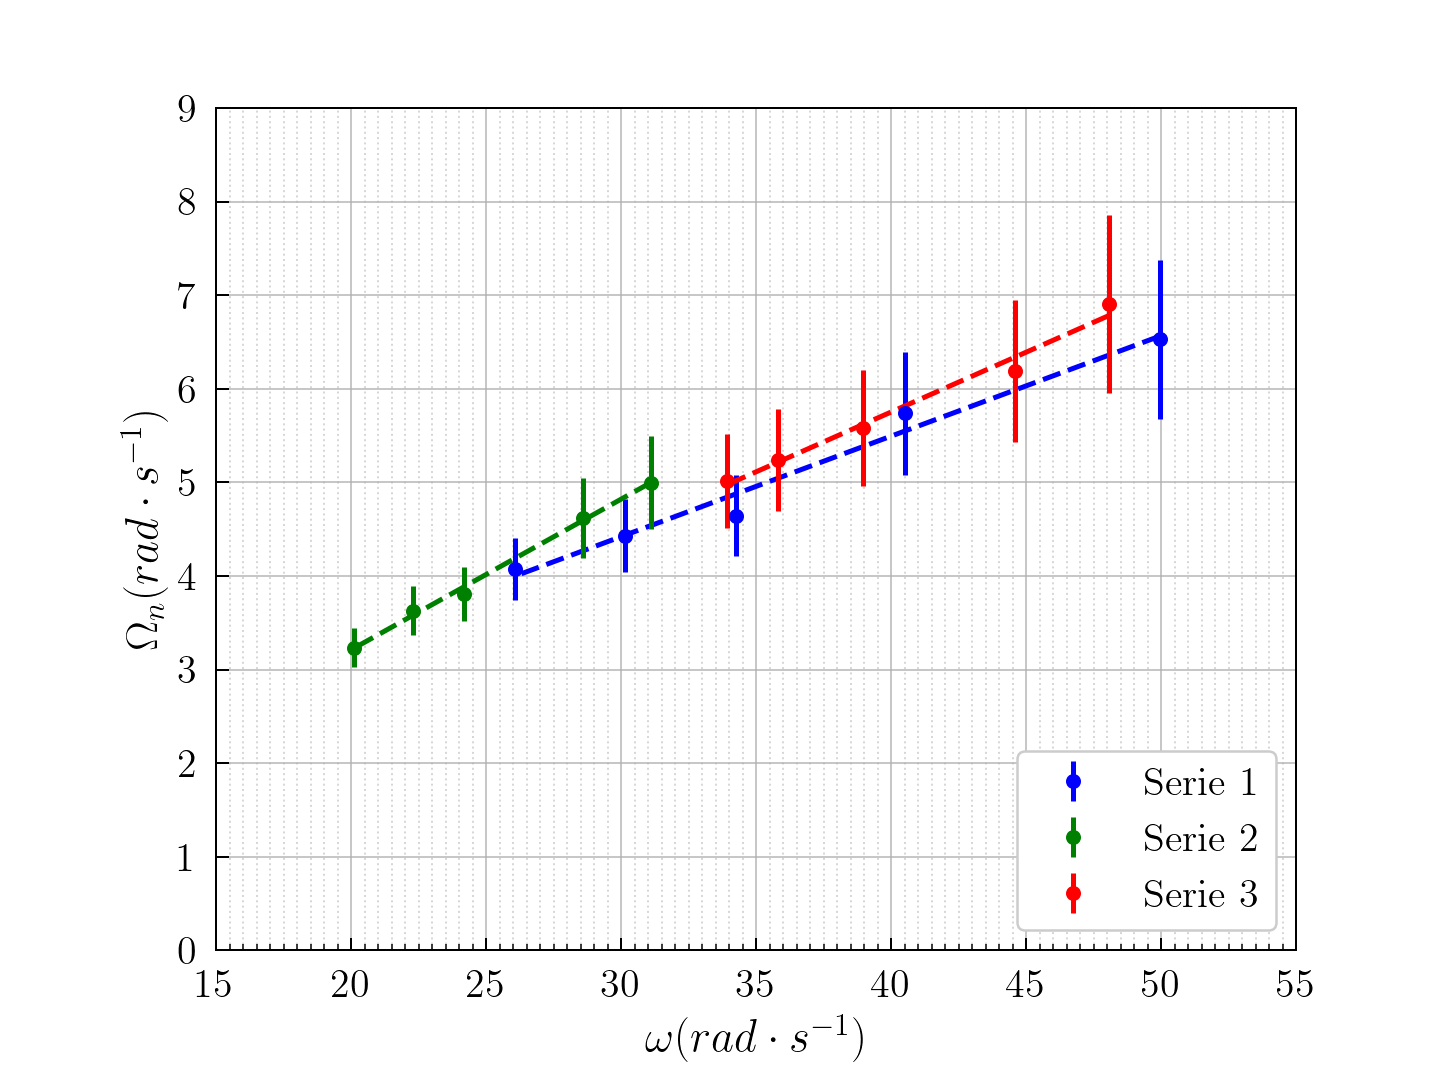
\includegraphics[width=0.75\linewidth]{Images/reg_nutacion2.png}
    \caption{Regresión lineal de $\Omega_n$ frente a $\omega$}
\end{figure}

\begin{table}[h!]
    \centering
    \begin{tabular}{|c|c|c|c|c|}
        \hline
        Parámetros & $a(rad\cdot s^{-1})$ & $b$ & $r$ & $I_1(kg\cdot m^2)$ \\ \hline
        Serie 1 & $1,20 \pm 0,35$ & $0,1074\pm 0,0096$ & 0,98 & $0,132 \pm 0,012$\\ \hline
        Serie 2 & $-0,01 \pm 0,15$ & $0,1609 \pm 0,0060$ & 0,997 & $0,0879 \pm 0,0033$\\ \hline
        Serie 3 & $0,64 \pm 0,40$ & $0,1278 \pm 0,0098$ & 0,991 & $0,1107 \pm 0,0085$\\ \hline
    \end{tabular}
    \caption{Parámetros obtenidos a partir de los ajustes}
\end{table}

\newpage

Los valores de $I_1$ son obtenidos a partir de la pendiente de la recta de regresión ($\Omega_n=a+b\omega$):

\begin{equation}
    b = \frac{I_3}{I_1} \Rightarrow I_1 = \frac{I_3}{b}
\end{equation}

Donde el valor de $I_3$ empleado será el calculado de forma teórica, por ser el que más se aproxima a la realidad. Con estos tres valores de $I_1$ vamos a calcular su media ponderada para obtener un valor de referencia:

\begin{equation}
    I_1 = 0,0936 \pm 0,0030 \;kg\cdot m^2
\end{equation}

\section{Conclusiones}

El giroscopio es un elemento en el que podemos apreciar perfectamente los conceptos de torque y momento angular, provocando resultados a priori inesperados como vimos en la primera parte de la práctica. En la segunda parte calculamos los momentos de inercia respecto a dos ejes, el de simetría y uno perpendicular a este. Los resultados se pueden ver en la siguiente tabla:

\begin{table}[h!]
    \centering
    \begin{tabular}{|cc|cc|}
    \hline
    \multicolumn{2}{|c|}{$I_3(kg\cdot m^2)$}                  & \multicolumn{2}{c|}{$I_1(kg\cdot m^2)$}                 \\ \hline
    \multicolumn{1}{|c|}{Teórico}     & $0,01415 \pm 0,00011$ & \multicolumn{1}{c|}{Teórico}      & $0,0625 \pm 0,0059$ \\ \hline
    \multicolumn{1}{|c|}{Caída libre} & $0,00963 \pm 0,00053$ & \multicolumn{1}{c|}{Oscilaciones} & $0,0791 \pm 0,0093$ \\ \hline
    \multicolumn{1}{|c|}{Precesión}   & $0,00447 \pm 0,00010$ & \multicolumn{1}{c|}{Nutación}     & $0,0938 \pm 0,0030$ \\ \hline
    \end{tabular}
    \caption{Resumen de los momentos de inercia calculados}
    \label{tab:my-table}
    \end{table}

En los resultados de $I_3$ podemos ver pequeñas diferencias entre el valor teórico esperado y los medidos experimentalmente. Esta diferencia se nota especialmente en el caso de la precesión, algo que era esperable en esta parte debido al gran factor humano que se ve implicado en la toma de medidas. Cabe destacar también la gran incertidumbre relativa de esta medida, tiene casi la misma que el valor teórico pese a que el valor de $I_3$ está un orden de magnitud por debajo. 
\par En los resultados de $I_1$ podemos ver que todos los valores están en el mismo orden de magnitud, difiere algo más el valor obtenido a partir del estudio de la nutación. Este valor, al igual que el obtenido por la precesión, era esperable que se alejara un poco de la realidad debida a la poca precisión que mostró el tacómetro en la toma de medidas. Una posible forma de obtener un mejor valor para $I_1$ en la nutación es no suponer que $s(\Omega_n)$ es constante y realizar un ajuste ponderado. Por último cabe destacar que el $I_1$ obtenido por nutación depende también de $I_3$, en concreto elegimos el valor teórico por ser el que creíamos más fiable pero el resultado se verá influído por el valor de $I_3$ tomado para hacer los cálculos.



\end{document}